\documentclass[border=6pt]{standalone}
\usepackage[T1]{fontenc}
\usepackage[utf8]{inputenc}
\usepackage[scaled=0.98]{helvet}
\renewcommand{\familydefault}{\sfdefault}
\usepackage{amsmath}
\usepackage{graphicx}
\graphicspath{{../../../../../../exercises_lecturenotes/lecture_notes/kurs100_lektionsnoter/}}
\usepackage{tikz}
\usepackage{pgfplots}
\pgfplotsset{compat=1.18}
\usetikzlibrary{arrows.meta, decorations.pathreplacing, calc, positioning, fit, backgrounds, shapes.geometric}
\usepgfplotslibrary{groupplots,fillbetween}
\definecolor{scanpink}{HTML}{E5006D}
\definecolor{scanteal}{HTML}{00A6A6}
\definecolor{scannavy}{HTML}{243746}
\definecolor{scanlightgray}{HTML}{F1F2F3}
\begin{document}
    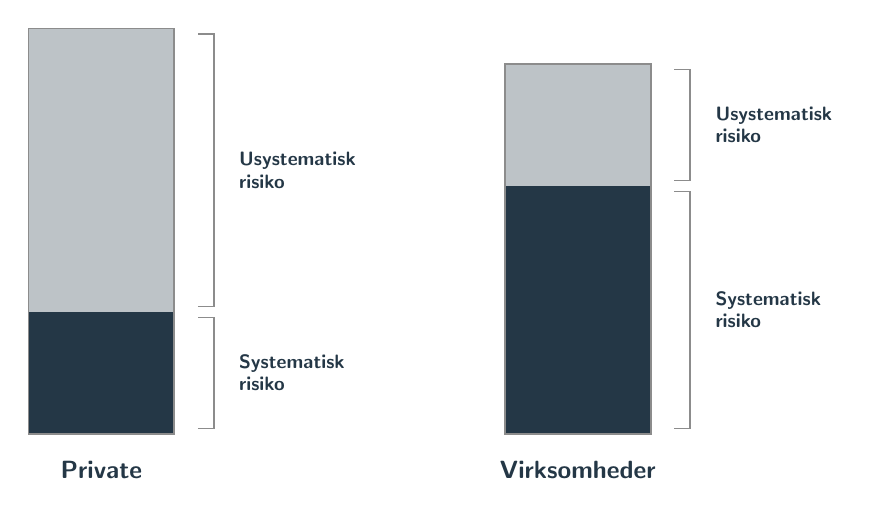
\begin{tikzpicture}[
        x=1cm,
        y=1cm,
        font=\small,
        baroutline/.style={
            draw=black!45,
            line width=0.65pt
        },
        riskbrace/.style={
            draw=black!45,
            line width=0.65pt
        }
    ]

        % Private: relativt stor usystematisk risiko
        \path[fill=scannavy]
            (0,0) rectangle (1.85,1.55);
        \path[fill=scannavy!30]
            (0,1.55) rectangle (1.85,5.15);
        \draw[baroutline]
            (0,0) rectangle (1.85,5.15);

        % Virksomheder: relativt stor systematisk risiko
        \path[fill=scannavy]
            (6.05,0) rectangle (7.90,3.15);
        \path[fill=scannavy!30]
            (6.05,3.15) rectangle (7.90,4.70);
        \draw[baroutline]
            (6.05,0) rectangle (7.90,4.70);

        % Klammer og betegnelser: private
        \draw[riskbrace]
            (2.15,1.62) --
            (2.35,1.62) --
            (2.35,5.08) --
            (2.15,5.08);

        \node[
            anchor=west,
            align=left,
            text=scannavy,
            font=\scriptsize\bfseries
        ] at (2.55,3.35)
            {Usystematisk\\risiko};

        \draw[riskbrace]
            (2.15,0.07) --
            (2.35,0.07) --
            (2.35,1.48) --
            (2.15,1.48);

        \node[
            anchor=west,
            align=left,
            text=scannavy,
            font=\scriptsize\bfseries
        ] at (2.55,0.78)
            {Systematisk\\risiko};

        % Klammer og betegnelser: virksomheder
        \draw[riskbrace]
            (8.20,3.22) --
            (8.40,3.22) --
            (8.40,4.63) --
            (8.20,4.63);

        \node[
            anchor=west,
            align=left,
            text=scannavy,
            font=\scriptsize\bfseries
        ] at (8.60,3.93)
            {Usystematisk\\risiko};

        \draw[riskbrace]
            (8.20,0.07) --
            (8.40,0.07) --
            (8.40,3.08) --
            (8.20,3.08);

        \node[
            anchor=west,
            align=left,
            text=scannavy,
            font=\scriptsize\bfseries
        ] at (8.60,1.58)
            {Systematisk\\risiko};

        % Kategorier
        \node[
            font=\small\bfseries,
            text=scannavy,
            anchor=north
        ] at (0.925,-0.22)
            {Private};

        \node[
            font=\small\bfseries,
            text=scannavy,
            anchor=north
        ] at (6.975,-0.22)
            {Virksomheder};

    \end{tikzpicture}
\end{document}
